\documentclass[11pt]{article}

\usepackage[final]{acl}
% Download the ACL style files from the link below.
% You need the `acl.sty' and `acl_natbib.bst' files, keep these in the same
% directory as your TeX file.
% https://github.com/acl-org/acl-style-files/tree/master/latex

\usepackage{times}
\usepackage{latexsym}
\usepackage[T1]{fontenc}
\usepackage[utf8]{inputenc}
\usepackage{microtype}
\usepackage{inconsolata}
\usepackage{hyperref}
\usepackage{graphicx}


\title{SemEval - Fine-tuning LLM for sentiment classification}

\author{Andrey Sypachev \\
  5126511\\
  M1101-CMS72 \\
  \\\And
  Long Tran \\
  5192922\\
  M1101-CMS72 \\
  \\}


\begin{document}
\maketitle
\begin{abstract}
Why do language models need to recognize human emotions?
When we read messages, posts or emails, we can easily miss important nuances of the author's mood and attitude towards a situation. If we understand the emotional coloring of a text, we can more accurately interpret the meaning and establish a closer connection with the person who wrote the message. Without recognizing emotions, we lose some of the context that affects the depth of communication. Communicating via chat can be a source of stress or, on the contrary, support. Recognizing the emotional coloring of the text helps to notice in time that someone may need help, support or at least a kind word. For example, algorithms that detect signs of depression in posts can help to intervene in time and suggest a person to consult a specialist [1]. Thanks to recognizing human emotions, we become more attentive and sensitive to the world around us. This makes life richer, brighter and more meaningful.

This report focuses on describing the fine-tuning process of existing language models for emotion recognition on an English text dataset.

\end{abstract}

\section{Introduction}

Human communication is inherently complex, and we frequently use language in indirect ways to express our emotions. We might say one thing while meaning another, particularly when dealing with sensitive topics, criticism and making jokes. This discrepancy between literal words and intended emotional meaning makes accurately guessing someone's emotional state a significant challenge. Oral communication's emotional interpretation is already challenging, interpretation of written text is even more problematic due to missing tones and facial expressions. Furthermore, individuals vary in how they express and perceive emotions, adding another layer of complexity. One person's innocent comment might be interpreted as offensive by another. Therefore, we can never be entirely certain about the true emotions of someone behind a written message.

While the task of understanding emotions expressed in texts can be framed as a multi-label classification problem, where multiple emotions might be present simultaneously, the real difficulty lies in the subtle difference between the sentiment expressed in the text itself and the actual emotion being felt by the speaker. Words may express one emotion, but the tone of voice or context might express another. To attempt to aid humans in sentiment detection in texts, we fine-tune the \textit{large language model} (LLM) BERT, in particular, BERT-large to classify text snippets by emotions: \textit{joy, sadness, fear, anger,} and \textit{surprise}. In section 2, we will mention the different models involved in our experiments. In section 3, we describe in detail the different models and the training parameters we experimented on. Next, in section 4, we evaluate the results produced by different models and the effects of the parameters described in the previous section, judging by the \textit{F-score}. After that, we will discuss what other methods can potentially be applied to further improve the score and fine-tune the model more efficiently for the \textit{multi-label text classification task}.

Our project can be accessed via this \href{https://github.com/KomaR1/TUD_SemEval_a/tree/main}{Link.}

\section{Methodology}
In this section, we will describe the fine-tuning process, technology and necessary components used during the process.

We apply the \textit{Hugging Face} library to achieve efficiency while maintaining simplicity. A fixed dataset was acquired from an external source. The dataset is then tokenized and split into smaller fractions for training and evaluation. A pretrained LLM model is then selected from \textit{Hugging Face} library. Next, we conducted experiments on several training arguments and saved the LLM model with the best F-score. After that, the fine-tuned model is used to perform test prediction on examples.
\subsection{Dataset}
The dataset used for training and fine-tuning was acquired from \textit{Codabench}, an open-source platform allowing you to organize AI benchmarks. There are 2768 rows in the train dataset. For each row, there are seven columns: \textit{id, text, anger, fear, joy, sadness,} and \textit{surprise}. The text column contains a set of random sentences of different lengths. The other five sentiment columns are labelled in binary value, indicating whether a text may express such emotions.

After being loaded from the CSV file, the original train dataset is split with the ratio 80/20 into two smaller parts, \textit{train data} and \textit{test data}, respectively. The text of each dataset is then proceeded to be tokenized by \textit{BertTokenizer}, a tokenizer specialised for BERT already built in \textit{Hugging Face} library. The sentiment label columns are combined into one label column and re-attached to the tokenized texts. At this stage, we have a tokenized train and test dataset ready to be plugged in for fine-tuning.
\subsection{Pre-trained Model}
Why was it in favor of BERT transformers? BERT's architecture is based on bidirectional transformers, and through them, the model can consider both left and right contextual information for any word. This is particularly important for sentiment analysis, in which meaning and emotion conveyed through a word will depend a lot on its surrounding context in a sentence. With its ability to consider contextual information, the model can discern the nuance in emotional shades [2].

BERT is initially trained with a large volume of texts, allowing the model to gain a lot of language-related information. When being fine-tuned for a target task (e.g., emotion classification), the model can adapt with ease and obtain high accuracy. The transfer of such information reduces enormously the amount of labelled information that must be present in order to obtain a satisfactory performance.

BERT is successfully utilized in a variety of tasks, such as sentiment analysis, named-entity recognition, question and answer, and many others. Several studies have confirmed that fine-tuned BERT models have outstanding performance even in multi-class classification tasks, in which a single text can have a variety of feelings [3]. Following the publication of the first BERT paper, several studies have successfully utilized the model in terms of sentiment analysis in a text, confirming its usability and efficiency for deep analysis of a text in terms of requirements [4]. Most present studies and NLP implementations use BERT for processes that demand a high analysis of the emotional facet

The choice of BERT arises out of its ability for complex contextual dependencies, high adaptability when fine-tuning over specific datasets, and success in works relating to deep text understanding, proven in many experiments. All of these make one of the most efficient tools for emotion recognition in texts out of BERT.
Prior to selecting a pretrained model, a performance comparison of accessible models of the family of BERT was conducted. As seen in the best experiments in Table 1, we have opted for the use of the BERT-large cased model.
\subsection{Training Arguments}
Our team’s fine-tuning process mainly focuses on the \textit{training arguments} to tweak the training process and produce the best F-score, while lowering the possibility of overfitting. Below is the combination of arguments that help us achieve the best possible score. 

\textbf{learning rate: $3\mathrm{e}{-5}$.} The initial learning rate for \textit{AdamW} optimizer. The optimizer adjusts the model’s weights to minimize the loss functions. The learning rate value determines the step size the optimizer takes when updating the weights [5]. The operation is somewhat similar to gradient descent. If the value is too high, the adjustment per epoch may overshoot the global optimum. If the value is too low, the convergence is slow, the model may get stuck in a local optimum, and fail to reach the best results before the training ends. 

\textbf{num\_train\_epochs: 15.} \textit{The number of epochs} is a hyperparameter that defines the number of times that the learning algorithm will work through the entire training dataset [6]. Empirically, a threshold of 15 epochs was established. On average, the model reaches its best result at epoch 11. In the case of bert-large-cased, the model achieves the best F-score at epoch 7. The training was halted automatically to prevent overfitting by setting \textit{early\_stopping\_patience=2}, which stops the training if the evaluation loss increases 2 epochs continuously. 

\textbf{per\_device\_train\_batch\_size: 16 and per\_device\_eval\_batch\_size: 16.} The \textit{batch size} is a hyperparameter that defines the number of samples to work through before updating the internal model parameters [7]. A batch size of 16 for both training and evaluation allows balanced GPU resource usage and maintains stable gradient descent without exceeding available RAM.

\textbf{warmup\_step: 1000.} The number of steps used for a linear warmup from 0 to learning\_rate, takes place during the warmup phase. Specifying 1000 warm-up steps reduces the initial instability of training, ensuring a smooth start to the optimization process. This warmup allows the model to stabilize and learn the basic patterns before being subjected to larger learning rates.

\textbf{lr\_scheduler\_type: linear. }The scheduler type to use takes effect after the warmup phase. The use of a linear learning rate scheduler helps to gradually and linearly decrease the learning rate as training progresses. Starting with a higher learning rate the model quickly explores the loss landscape. As the model gets closer to the optimum, reducing the learning rate allows it to make finer adjustments to reach convergence and avoid overfitting.

\textbf{weight\_decay: 0.01}. A method of \textit{regularization} mainly to limit overfitting. A weight decay value of 0.01 is applied, which helps reduce the risk of overfitting by limiting the magnitude of the model’s weights.

\textbf{max\_grad\_norm: 1.0. }To improve the stability of the optimization process, \textit{gradient norm clipping} was used to prevent excessively large weight updates, avoiding “exploding gradient” problem. By setting the argument’s value to 1.0, the training process clips the gradients if their magnitude exceeds 1.0. 
Besides experimenting with the training arguments, we also set two arguments for the pretrained model itself.

\textbf{hidden\_dropout\_prob=0.2.} The \textit{dropout probability} for all fully connected layers in the embeddings, encoder, and pooler. When set to 0.2, each neuron in the hidden layers has a 20\% chance of being dropped out during each training step. Since the argument affects directly the weights and neuron participation, if measured correctly, this argument helps to achieve optimum. Otherwise, it may lead to underfitting if the value is too low, or overfitting if too high. [8]

\textbf{attention\_probs\_dropout\_prob=0.2.} Similar to \textit{hidden\_dropout\_prob}, this dropout ratio is for the \textit{attention probabilities}. 


\section{Evaluation}
This section contains quantitative and qualitative evaluations of the results of the pre-trained BERT model for emotion detection.
\subsection{Quantitative evaluation}
To evaluate its performance in a multi-class classification problem, we have used the following metrics:
\textbf{F1 Score} (F-score). The micro F1 score considers the overall true positive, false positive, and false negative values for all classes and is therefore particularly useful in cases of class imbalance. That the model is effective in identifying the nuanced emotion cues in the text is hinted at by its attained F1 value. The model consistently performed with an F1 value of approximately \textbf{0.77}, bearing witness to its accuracy in predicting emotion cues in the text in consideration of multi-label classification difficulty. An accuracy of approximately \textbf{0.5} reflects the difficulty in mapping predicted labels with ground truth perfectly in a multi-label scenario.

\textbf{Accuracy.} While accuracy is a universal metric, in multi-label classification of emotions, it can be less helpful because a text can convey multiple emotions. With an accuracy of around 0.5, it can imply that the model doesn't always predict the entire set of correct emotions, an issue that can arise in such a case.
\subsection{Qualitative evaluation}
In addition to quantitative analysis, we have also utilized the \textbf{SHAP} (SHapley Additive exPlanations) tool to comprehend the model’s decision-making mechanism. The individual contribution of a token towards overall prediction was analyzed through SHAP. The tool aids in knowing which parts of the text contribute most toward a specific emotion's classification. For example, through analysis with SHAP, one can observe that in a sentence describing extreme or emotionally charged situations, the model identifies relevant terms or words in a proper manner that correspond to a specific emotion.

The use of SHAP supports enhancing model interpretability and trust in its output. For emotion analysis use cases in text, algorithm transparency can go towards a deeper analysis of model behavior and future model improvement [9]. The SHAP analysis revealed that the model effectively considers significant terms and phrases that inform its prediction, and in doing so, it both confirms internal representations and interpretability. The results of the SHAP analysis are presented in Figure 1 and Figure 2.

\section{Discussion}
The fixed dataset was provided to us by Codabench with the size of 2768 rows, already cleaned and ready to use. This helped us save a lot of time and effort as it cut away the need to gather and clean the data and spend all the time available committing to fine-tuning the model. Additionally, the dataset has already been structured and included data that are necessary for a multi-label text classification task, potentially supporting in achieving the best fine-tuning results. Despite so, this eliminates the chance of utilizing and experimenting on datasets of larger sizes, disregarding their potential advantages as they can also improve the performance to a certain extent [10].

Hugging Face is a library dedicated to machine learning and generative AI. The library provides components such as transformers, tokenizers, and, most importantly, pretrained models and trainers. Despite the impediment on flexibility and robustness, the library allows us to significantly streamline and accelerate our fine-tuning task. With the use of trainers, we eliminate the need for manual configuration for each epoch and, instead, only specify training arguments and pass them to the trainer. Furthermore, using a pretrained model and implementing components from the same library and framework will benefit the training process and result in more promising performance. 

In summary, we were able to fine-tune a pretrained BERT-large model to perform a multi-label text classification task, detecting sentiment from text. The dataset provided by Codabench allows us to invest our time in the fine-tuning process. For the process, we implemented Hugging Face library to streamline our experiment and train the model more effectively. Finally, we decided to conclude our experiment as we have achieved a bert-large-cased model with an F-score of \textbf{77}, the best among those we experimented on.
\section{Reference}
[1] Cao, Y., Dai, J., Wang, Z., Zhang, Y., Shen, X., Liu, Y., \& Tian, Y. (2024). Systematic Review: Text Processing Algorithms in Machine Learning and Deep Learning for Mental Health Detection on Social Media. arXiv preprint arXiv:2410.16204.

[2] Devlin, J. (2018). Bert: Pre-training of deep bidirectional transformers for language understanding. arXiv preprint arXiv:1810.04805.

[3] Sun, C., Qiu, X., Xu, Y., \& Huang, X. (2019). How to fine-tune bert for text classification?. In Chinese computational linguistics: 18th China national conference, CCL 2019, Kunming, China, October 18–20, 2019, proceedings 18 (pp. 194-206). Springer International Publishing.

[4] Liu, Y. (2019). Roberta: A robustly optimized bert pretraining approach. arXiv preprint arXiv:1907.11692, 364.

[5] Yuan, J. (2024). Performance Analysis of Deep Learning Algorithms Implemented Using PyTorch in Image Recognition. Procedia Computer Science, 247, 61-69.

[6] Brownlee, J. (2018). What is the Difference Between a Batch and an Epoch in a Neural Network. Machine learning mastery, 20, 1-5.

[7] Yedida, R., \& Saha, S. (2019). A novel adaptive learning rate scheduler for deep neural networks. arXiv preprint arXiv:1902.07399.

[8] Srivastava, N. (2013). Improving neural networks with dropout. University of Toronto, 182(566), 7.

[9] Lundberg, S. M., Lee, S.-I. (2017). A Unified Approach to Interpreting Model Predictions. arXiv preprint arXiv:1705.07874.

[10] Prusa, J., Khoshgoftaar, T. M., \& Seliya, N. (2015, December). The effect of dataset size on training tweet sentiment classifiers. In 2015 IEEE 14th International Conference on Machine Learning and Applications (ICMLA) (pp. 96-102). IEEE.

\clearpage
\onecolumn
\section{Appendix}

\begin{table}[htp]
\caption{BERT performance comparison}
\centering
\begin{tabular}{|l|l|l|l|}
\hline
\textbf{Model} & \textbf{Training Loss} & \textbf{Validation Loss} & \textbf{F1-score} \\ \hline
distilbert-base-cased   & 22.7 & 39.7 & 71.5 \\ \hline
distilbert-base-uncased & 32.6 & 38.6 & 71.4 \\ \hline
bert-base-cased         & 22.7 & 39.4 & 74.1 \\ \hline
bert-base-uncased       & 24.4 & 37.0 & 74.0 \\ \hline
bert-large-cased        & 17.4 & \textbf{36.6} & \textbf{77.0} \\ \hline
bert-large-uncased      & \textbf{16.0} & 39.3 & 75.2 \\ \hline
\end{tabular}
\label{tab:bert_performance}
\end{table}

\begin{figure}[htp]
    \centering
    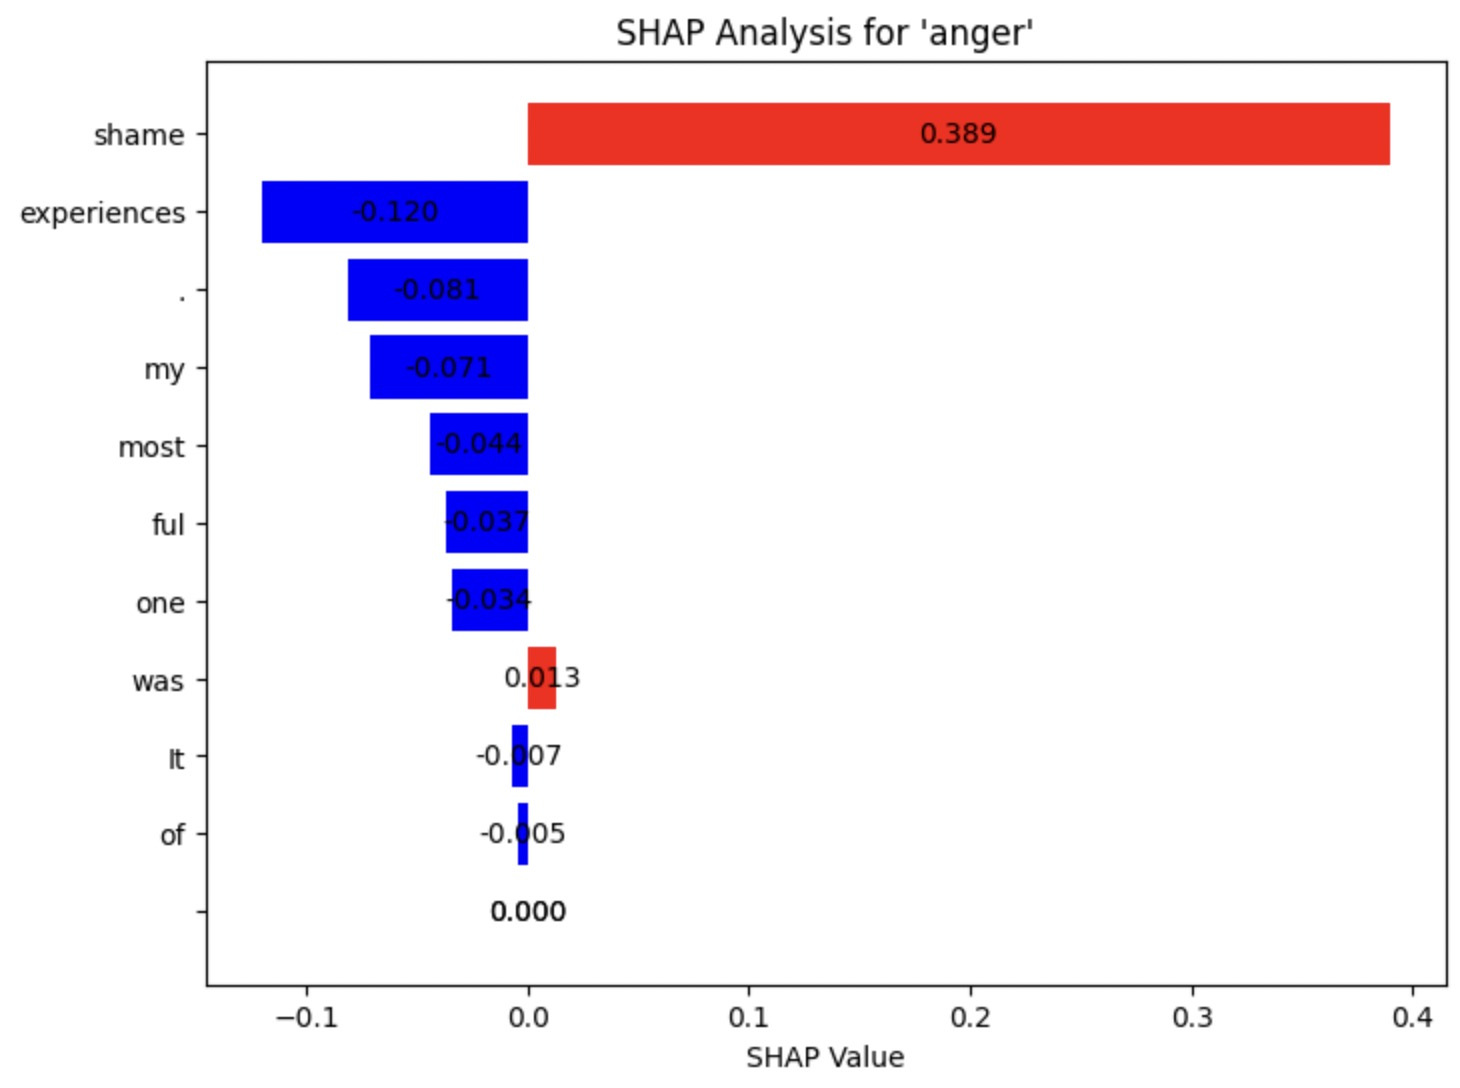
\includegraphics[width=0.8\linewidth]{images/figure1.jpg}
    \caption{SHAP analysis result of the 3rd sentence in the test dataset for the label “anger”}
    \label{fig:figure1}
\end{figure}

\begin{figure}[htp]
    \centering
    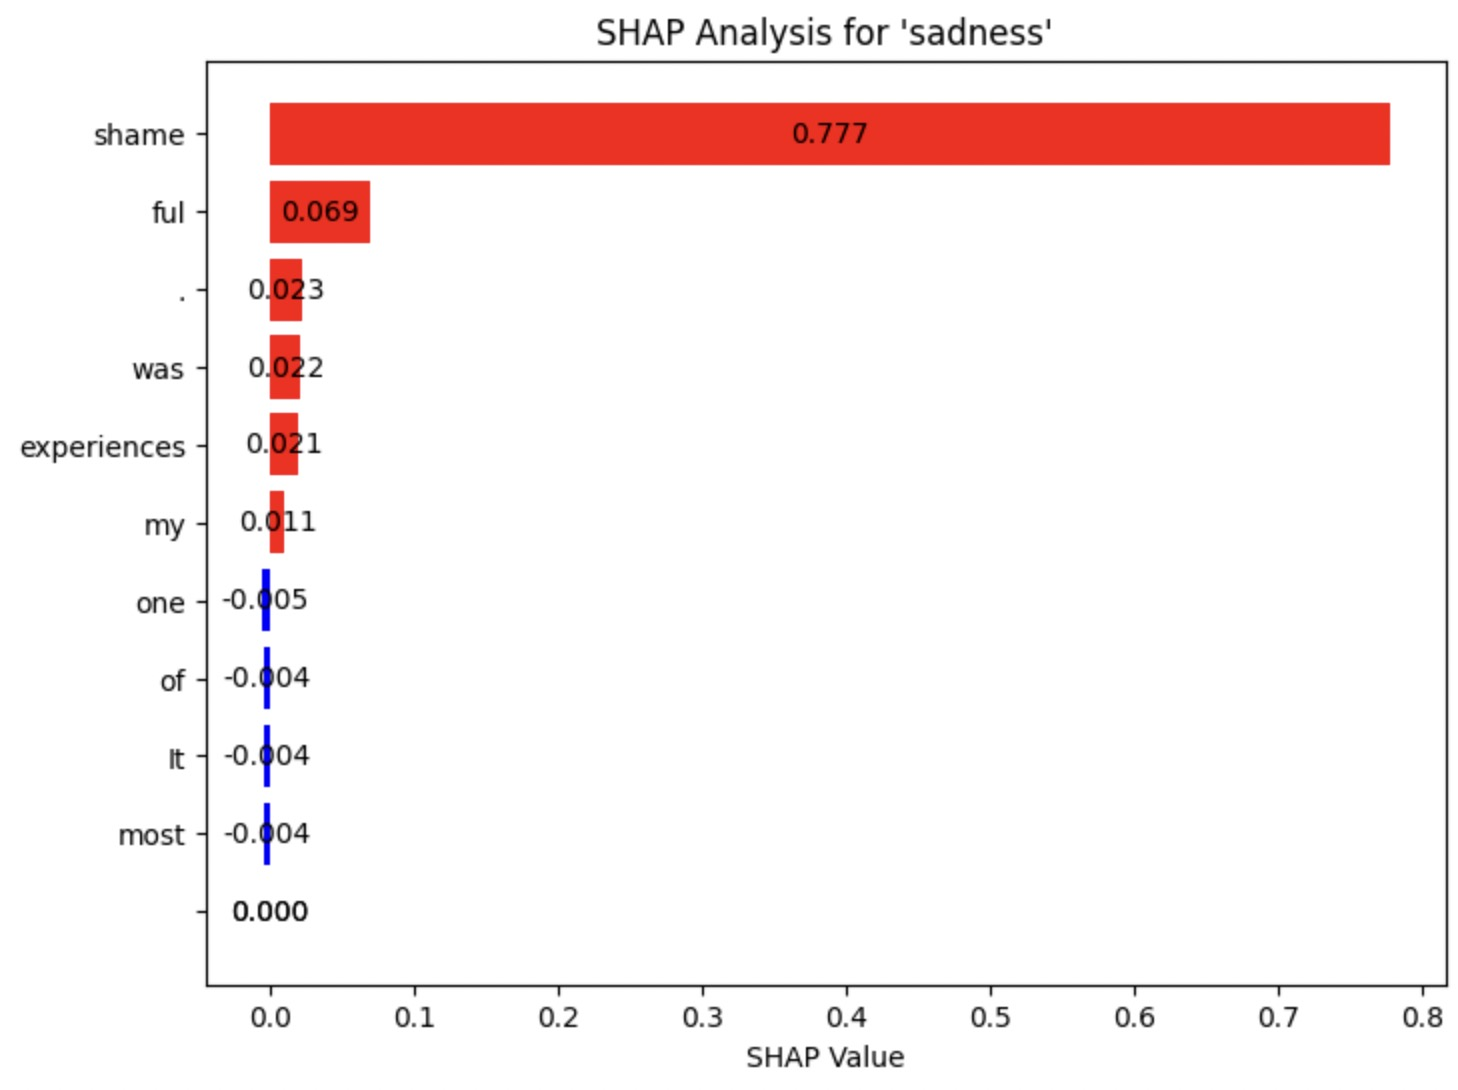
\includegraphics[width=0.8\linewidth]{images/figure2.jpg}
    \caption{SHAP analysis result of the 3rd sentence in the test dataset for the label “sadness”}
    \label{fig:figure2}
\end{figure}

\clearpage
\twocolumn


\end{document}
